\RequirePackage[hyphens]{url}

\documentclass[sigconf]{acmart}

\usepackage{graphicx}
\usepackage{hyperref}
\usepackage{todonotes}

\usepackage{endfloat}
\renewcommand{\efloatseparator}{\mbox{}} % no new page between figures

\usepackage{booktabs} % For formal tables

\settopmatter{printacmref=false} % Removes citation information below abstract
\renewcommand\footnotetextcopyrightpermission[1]{} % removes footnote with conference information in first column
\pagestyle{plain} % removes running headers

\newcommand{\TODO}[1]{\todo[inline]{#1}}
\newcommand{\DONE}[1]{DONE: \todo[inline,color=green!30]{#1}}


\begin{document}
\title{Can Blockchain Adoption Mitigate the Opioid Crisis Through More Secure Drug Distribution?}


\author{Saurabh Kumar}
\affiliation{%
  \institution{Indiana University}
  \city{Bloomington} 
  \state{IN} 
  \postcode{47408}
  \country{USA}}
\email{kumarsau@iu.edu}

\author{Mathew Schwartzer}
\affiliation{%
  \institution{Indiana University}
  \city{Bloomington} 
  \state{IN} 
  \postcode{47408}
  \country{USA}}
\email{mabschwa@iu.edu}

\author{Nicholas J Hotz}
\affiliation{%
  \institution{Indiana University}
  \city{Bloomington} 
  \state{IN} 
  \postcode{47408}
  \country{USA}}
\email{nhotz@iu.edu}

\begin{abstract}
Like TCP/IP in the 1970s and 1980s, blockchain is a new, intriguing but grossly misunderstood technology that is still in its infancy. It is commonly misunderstood as just a technology for Bitcoin and cryptocurrencies. However, blockchain's use cases extend beyond just financial transactions and cryptocurrencies, and have the potential to transform nearly every industry including healthcare and supply chain. As the technology matures, additional transformative use cases could expand into drug distribution and specifically to opioid supply chains. Despite this potential, a publicly-available blockchain specifically for opioid supply chains was not found. Therefore, to demonstrate how a blockchain would function on a simplified opioid supply chain, a blockchain, using Python code, was developed as a proof of concept. This source code is publicly available to allow others to further develop the blockchain model for more complex and real-world opioid supply chains. The collective review and analysis of blockchain, pharmaceutical supply chains, the opioid crisis, and the demonstrated blockchain model suggest that the adoption of blockchain systems for prescription opioid supply chains would enable numerous capabilities that could mitigate certain aspects of the opioid crisis.
\end{abstract}

\keywords{HID 210, HID 212, HID 225, i523, blockchain, opioid epidemic, pharmaceutical supply chain, healthcare}

\maketitle

\section{Introduction}
\subsection{The Need to Modernize Global Record Keeping}
Contracts, transactional records, and verification systems are part of the foundational core of the global economy. However, as Iansiti and Lakhani \cite{hbr} explain, these tools have not modernized to keep up with the needs of the rapidly evolving global economy and are ``like a rush-hour gridlock trapping a Formula 1 car.'' Records and transactions are still being managed as they were in the 20th century which creates broad consequences for nearly every industry including supply chain and healthcare.

In supply chain, data management methods for records and logistics are usually inconsistent across the different levels of a supply chain \cite{arbc4}. The outdated record management method encourages redundant data to be stored at the same organization as well as across the supply chain which increases IT maintenance costs and decreases trust and transparency \cite{arbc1}. These issues prevent a tertiary party, like the government, to effectively scrutinize records. 

Outdated data management processes also negatively impact healthcare. In the USA in 2014 healthcare fraud cost an estimated \$272 billion \cite{economist2014}, and in 2016, healthcare data breaches impacted over 27 million patients \cite{das2017}. Today, medical data management is stifled by antiquated technology that limits patients' ability to manage and control access to their electronic medical records \cite{ekblaw2016medrec}.

In addition, pharmaceutical supply chains are enervated by current record-keeping technologies. Transactional records are rarely shared across pharmaceutical supply chain organizations which consequently increases inventory levels \cite{Nematollahi01}. As a result, total healthcare cost and the opportunity for counterfeit drugs increases \cite{Sahay01}. In addition, verification systems are often independent among supply chain retailers and prescribers. The lack coordination opens the door for ``doctor shopping'' and greater prescription medication abuse \cite{hitchingHealthcare}. 

\subsection{Rational Exuberance for Blockchain}
The adoption of blockchain, ``an open, distributed ledger that can record transactions between two parties efficiently and in a verifiable and permanent way'' \cite{hbr}, has the potential to resolve these and other fundamental problems of the global economy by overcoming many of the antiquated shortcomings of the traditional means of managing and verifying contracts and transactions. However, like TCP/IP in the 1970s and 1980s, blockchain is an immature technology that faces numerous challenges to mass adoption. In spite of its current limitations, blockchain is already seeing promising applications in various industries extending beyond just finance including healthcare and supply chain.

One particularly exciting use case sits at the intersection of healthcare and supply chain. Blockchain could provide a more secure distribution system for opioid medications that would develop enabling and foundational capabilities that would potentially mitigate certain aspects of the opioid crisis. To further develop and evaluate this potential use case, a blockchain model based on a simplified pharmaceutical supply is presented with publicly-available source code for further development.





\section{Blockchain Overview}
Blockchain's secure distributed ledger framework includes three data types and has the potential to deliver numerous benefits but faces major hurdles toward mass adoption. Proper application of design principles can overcome these hurdles and accelerate the realization of these benefits.

\subsection{The Blockchain Framework}
Blockchain is a foundational technology comprised of numerous technological processes and entities \cite{hbr}. Some of the most significant pieces follow.

\subsubsection{Node} Nodes are the individual units connected to the blockchain network. They are computers with adequate software to maintain a blockchain. The blockchain network connects all the nodes and can read and write data to a block \cite{pabc1} \cite{pabc2}.

\subsubsection{Block} Blocks are the group of records, bundled together by nodes. They follow a specific set of rules and have limited size. Blocks are also linked to the last generated block, thus forming a chain \cite{pabc1}.

\subsubsection{Smart Contracts} Smart contracts are the codes with timestamps to represent a contract \cite{pabc1}. Iansiti and Lakhani \cite{hbr} believe that ``'smart contracts' may be the most transformative blockchain application at the moment,'' because they allow for automatic payments whenever contract conditions are met. 

\subsubsection{Submit Transaction} In case of a new transaction submission to the network, an individual node circulates it to all the other nodes in the network \cite{pabc1}. The main purpose of circulation is approval. 

\subsubsection{Transaction Approval} When a transaction is submitted and circulated in the network, each node verifies it. Invalid transactions are deleted \cite{pabc1}.

\subsubsection{Consensus} For multiple systems to work in a distributed network, they must have an agreement. Such a structure is useful in case of fault tolerance when those agreed set of protocols help to restore the data \cite{pabc1}.

\subsection{Data Types in Blockchain}
There are three major types of data stored on a blockchain, namely un-encrypted, encrypted, and hashed \cite{arbc1}. 

\subsubsection{Un-encrypted Data} All the organizations have read access to the un-encrypted data. Such data is fully transparent and facilitates immediate dispute resolution \cite{arbc1}.

\subsubsection{Encrypted Data} The encrypted data can only be read by the organizations with the access to such data. This means an organization should have a decryption key to read to read the encrypted data. Encrypted data provides restricted access but is also stored in every node in the blockchain. In case of a dispute, the decryption key could be used by different organizations to rectify the entry or deletion of any record \cite{arbc1}.

\subsubsection{Hash Data} Hash data is also a hidden data type, where hash keys act like fingerprints to represent changes or entry for any data record. Each organization can easily confirm their hash keys. Breaking the hash key is nearly impossible. Only the hash key is in the blockchain while the record data is stored off-chain by individual organizations. Data could be revealed, in case of a dispute, by the respective organization \cite{arbc1}.

\subsection{Benefits of Blockchain}
The exuberance surrounding blockchain stems from the fundamental benefits that are cornerstones to nearly every industry.

\subsubsection{Trust} Blockchains enable parties that do not know each other to trust each other. No single organization is trusted to maintain the records. Instead, all organizations must approve the contents of the record in order to avoid disputes. Therefore, records should have a timestamp and an origin proof. Normally, a third party facilitates this requirement. Blockchains can provide an alternate solution, where organizations jointly manage the records and preventing corruption by a single organization \cite{arbc1}. 

\subsubsection{Access} Blockchains allow for greater control over what information is and is not accessible. The technology enforces identical data to be stored by each organization. When one copy is updated, all the other copies are also updated. This eliminates the need for a third party to facilitate management of records \cite{arbc3}. Alternatively, different levels of read and write access could be provided to different organizations. Although some meta data should be stored in the public ledger. 

\subsubsection{Redundancy} Blockchain also assists in providing security by disallowing redundancy at the same node. The core logic of blockchain does not allow duplicate entries to be created in the same place which obviates the risk of duplicate entry, either intentional or accidental \cite{arbc4}.  For example, one of the major benefits of Bitcoin is that the same coins can be spent in multiple places, overcoming the so-called  ``double spend'' problem \cite{tapscott}.

\subsubsection{Transparency} Transparency in a business helps to grow trust among organizations. Sharing information can improve relationships among these organizations. Without blockchain, transparency is hard to achieve. Blockchains can help improve the visibility of contracts, legal documents as well as other inter-organization data \cite{pabc1}. Organizations are not obligated to show all of their data. Varying levels of access can be provided for data that could be useful to other organizations and a shared collection of records can also be stored and managed by co-operation from different organizations \cite{tapscott}.

\subsubsection{Low Transaction Costs} Through by-passing third-party verification systems such as brokers, lawyers, or banks, blockchain could significantly reduce transaction costs. Not only will this lower costs for existing transactions, it could open up the market for micro-payments \cite{hbr}. 

\subsection{Challenges to Blockchain Mass Adoption}
While blockchain adoption has the potential to help a wide variety of the world's problems, it should not be viewed as a panacea.  Blockchain is not mature enough to support mass-market adoption and faces numerous challenges. Rabah \cite{rabah2017overview} states that to be effective, blockchain needs to overcome its shortcomings of lacking standard protocols, unclear regulation, large energy and computing power consumption, privacy, cultural adoption, and high initial capital requirements. Tapscott and Tapscott \cite{tapscott} agree that its current technical infrastructure is not sufficient, its energy consumption and computational requirements are not sustainable, and user-friendly systems have yet to be designed that would allow for mass market adoption.

Society would have to dismantle many technological, governance, organizational, and cultural barriers to create new foundations for a new world economy that relies heavily on blockchain \cite{hbr}. This will come at the cost of some existing societal norms, core business functions, and people's jobs \cite{hbr} \cite{rabah2017overview}. 

\subsection{Technology Adoption Lifecycle}
Iansiti and Lakhani \cite{hbr} argue that the process for mass adoption of blockchain may take longer than expected but will follow a fairly predictable technology adoption pattern that parallels the adoption of TCP/IP (transmission control protocol / internet protocol). TCP/IP started as \textit{single-use} and matured to \textit{localized uses}, \textit{substitutions}, and \textit{transformations}. It was introduced as a \textit{single-use} in 1972 for e-mail in ARPAnet, a precursor to commercial internet for the US Department of Defense. Met with skepticism, this technology slowly gained traction among some firms in the 1980s and early 1990s for \textit{localized use} and did not become mainstream until the emergence of World Wide Web in the mid-1990s. This then paved the road for infrastructure companies to provide the necessary hardware and software to establish ``plumbing'' systems for the internet. Once the technical infrastructure was mature enough, companies then developed businesses that \textit{substituted} existing services with online services (such as Amazon books instead of Borders). Finally, a wave of companies created \textit{transformative} applications that fundamentally changed service experiences (such as Napster in the music industry or Skype in telecommunications).

Similarly, blockchain was also launched for a \textit{single use} in 2009 for Bitcoin, a virtual currency. Blockchain has matured to extend beyond cryptocurrencies and is now being applied for various \textit{localized uses} including in healthcare and supply chain. It took over 30 years for TCP/IP to realize its potential, and blockchain will likewise require decades to mature into a revolutionary economic force. However, companies can start planning for this revolution today and implement blockchains that follow seven key design principles \cite{hbr} \cite{tapscott}.

\subsection{Seven Design Principles for Blockchain}
Tapscott and Tapscott \cite{tapscott} in their book \textit{Blockchain Revolution} propose seven design principles that, when appropriately applied, can help blockchain move down the technology adoption lifecycle and create more honest, cost-effective, and accountable systems.

\subsubsection{Networked integrity} Because all organizations on the block\-chain must approve updates, ``Participants can exchange value directly with the expectation that the other party will act with integrity.'' \cite{tapscott}. 

\subsubsection{Distributed Power} Since the blockchain is distributed across a broad network, it cannot be dismantled by authoritarian power, hackers, or other bad actors. There are no single points of failure and the blockchain can still perpetuate even if numerous nodes are compromised \cite{tapscott}.

\subsubsection{Value as Incentive} Blockchains can align incentives of individual participants with the interests of the entire blockchain. This minimizes organization problems and conflicts of interests \cite{tapscott}.

\subsubsection{Security} Blockchains can protect against hackers, malware, ransomware, and identity theft by using a variety of security features. Public key infrastructures, private keys, public keys, and verification methods verify participant activities and prevent bad actors from overriding the network \cite{tapscott}. 

\subsubsection{Privacy} Blockchains can and should provide participants with the freedom to expose as little or as much information about themselves as they desire. This allows a participant to act anonymously when desired or to share sensitive information with only appropriate parties when needed \cite{tapscott}.

\subsubsection{Rights Preserved} To protect against counterfeit items, a blockchain can serve as a public ledger of ownership \cite{tapscott}.

\subsubsection{Inclusion} Currently, access to certain financial services is limited to those who are deemed ``creditworthy''. Blockchains can and should have significantly lower bars of entry that are not managed by banking institutions so that even a poor rural former on a remote corner of Earth who isn't creditworthy, could participate in the blockchain \cite{tapscott}.





\section{Blockchain Applications in Supply Chain and Healthcare}
In the broad public's view, blockchain is mostly known for Bitcoin; however, people are beginning to realize its potential to transform nearly every industry \cite{hbr}. Two such industries include supply chain and healthcare.

\subsection{Supply Chain}
Blockchain, being a public ledger, can be used in different domains with slight variation in its core attributes. While the general implementation says that the data of a single block is public to all the nodes, different sets of access rights could be provided to different classes of users.  Such implementation of blockchain could be applied to a supply chain network. 

A supply chain requires the involvement of various parties helping each other. This is generally a one-to-one chain network. Often, each organization uses different technologies for record keeping. Record keeping could involve any information ranging from direct communications to logistics. Trust is an important issue between organizations. Most of the organizations in a supply chain keep individual records, which are not public to other organizations in the supply chain. Organizations share some information like contracts or notarized data. An efficient management of such shared data can be accomplished using a blockchain. The blockchain provides the ability to collect, record, and notarize different types of shared data \cite{arbc1}. 

Blockchain could also facilitate storing and maintaining logistics data. Such an application could be useful in the field of healthcare, where the government wants to monitor the supply of drugs. By simplifying the storage and management of information, blockchain could provide easy access of such critical public sector information to government organizations while providing data security \cite{arbc2}. Blocks comprise of the data records. When these blocks are added to the chain, they become immutable. This means they cannot be deleted or changed by a single organization \cite{arbc2}. A consensus has to be reached by a majority of the organizations for changing any record. Such a feature helps to maintain the security of the records by eliminating data corruption. Each block is verified and managed using some shared protocols. This process can be automated to allow ease of data entry.

\subsection{Healthcare}
Representing over 17\% of the United States' GDP, healthcare costs continue to soar \cite{hitchingHealthcare}. Healthcare data in the United States reached 150 exabytes in 2011 with Kaiser Permanente, California's health network, reportedly having between 26.5 and 44 petabytes alone \cite{cottle2013transforming}. The volume of healthcare data is likewise soaring, doubling every 12-14 months \cite{dinov2016volume}, and the diversity of this data scattered across disparate systems further complicates its analysis \cite{frost2015drowning}. More effective data management could address many of healthcare's fundamental issues, and according to a 2011 McKinsey report \cite{mckinsey2011}, more effective health data management could save \$300 billion annually. Current innovations focus on placing patients at the center, privacy and access, completeness of information, and cost \cite{hitchingHealthcare}. Three interesting applications of blockchain for healthcare are in claims adjudication, cyber security and healthcare IoT, and electronic medical records \cite{das2017}.

\subsubsection{Claims Adjudication and Fraud Prevention}
The Economist \cite{economist2014} estimated that in 2014 the United States wasted \$272 billion dollars on healthcare fraud. Blockchain could not only minimize fraudulent billing; but, by automating claims adjudication and billing processes, obviate the need for administrative and transactional costs through third parties. Gem Health and Capital One are developing a blockchain-based solution for healthcare claims management \cite{das2017}.

\subsubsection{Cyber Security and Healthcare IoT}
In 2016, there were 450 reported health data breaches, impacting 27 million patients. Hacking and ransomware were responsible for 27\% of these breaches. Each additional connected medical device serves as a potential entry point for bad actors. With an estimated 20-30 billion healthcare IoT devices by 2020, blockchain could secure these devices and protect confidential data. Telstra, IBM, and Tierion are three companies that are developing cyber security solutions for connected healthcare devices \cite{das2017}.

\subsubsection{Electronic Medical Records} Beleaguered by stifled technology development, limited ownership control by patients, fragmented information systems, and risks of electronic protected health information hacking, electronic medical records have perhaps the most important use cases for blockchain \cite{yuan2016blockchains}. Blockchain can provide interoperability of healthcare information, improved security, patient-centric control, and immutable records \cite{das2017}. Three examples of blockchain-based EMRs include MedRec, Medicalchain, and the Estonian eHealth Foundation. First, by leveraging smart contracts on the Ethereum blockchain, MedRec is a prototype system that provides patients with ``one-stop-shop access to their medical history'' and shows promise to give ownership of health information back to the patients who can selectively share access through a modern API interface in a secure manner \cite{ekblaw2016medrec}. Second, Medicalchain is a permissioned blockchain distributed on networks of international healthcare providers that allow patients to transfer medical records across national borders \cite{hitchingHealthcare}. Third, a data security company called Guardtime is using its Keyless Signature Infrastructure system in partnership with the Estonian eHealth Foundation to store Estonian health records on a blockchain.





\section{The Opioid Crisis}
The United States opioid crisis is an overwhelming, tangled web of issues with increasingly severe health and financial consequences. The private sector, government, and academia are suggesting and implementing critical mitigation strategies to combat the crisis.

\subsection{Addiction Risk}
Since the late 1990s, pharmaceutical companies have downplayed the addictive risk of opioids \cite{opsis1}. However, the addictive nature of prescribed opioid painkillers increases the ``potential for unforeseen adverse events for the patient, including overdose, experience of physiological dependence and subsequent withdrawal, addiction, and negative impacts on functioning'' \cite{Vowles01}. Patients with wholesome medical intentions often fall victim to the pills' addictive nature. Misuse and eventual abuse of prescribed opioid painkillers is common: 21\%-29\% of patients prescribed opioids for chronic pain misuse them while 7.8\%-11.7\% develop an addiction \cite{Vowles01}. Moreover, an opioid addiction often serves as a gateway to other illegal drug use. With similar highs, prescription opioid addicts often transition to heroin, an illicit street-made opioid, since it is cheaper and easier to obtain. In fact, 4\%-6\% of patients using prescribed opioids develop a heroin addiction \cite{opsis1}. Whereas, 75\% of heroin users began their opioid addiction with prescription opioids \cite{Cicero01}.

Despite these risks, opioids are still prescribed at alarming rates. In fact, the United States, with about 5\% of the world's population, consumed 80\% of the world's opioid prescriptions from 2001-2010 \cite{Vowles01}. Between 1999 and 2015 the number of prescribed opioids painkillers such as codeine, fentanyl, oxycodone, Demerol, and Vicodin quadrupled. In the same time period, opioid-related deaths also quadrupled.
 
\subsection{Health Impact}
The epidemic has become so severe that in October 2017 President Trump was forced to declare it ``a national health emergency'' \cite{opsis3}. With no signs of stopping, this epidemic is burgeoning across America killing nearly 91 people a day \cite{opsis10}.
 
In 2015, 33,091 Americans died from an opioid overdose with rural white males at the greatest risk of an opioid overdose.  White Americans (27,056) died the most, followed by black Americans (2,741), and Hispanic Americans (2,507). Generally the middle-aged population was most at risk with the following percent mortality distributions by age group \cite{opsis4}:
\begin{itemize}
\item Aged 0-24: 10\% of the opioid-related deaths
\item 25-34: 26\% 
\item 35-44: 23\% 
\item 45-54: 23\% 
\item 55+: 19\% 
\end{itemize}
Males die nearly twice as frequently from an opioid overdose, representing 65\% deaths compared with 35\% for females \cite{opsis4}.

\subsection{Financial Impact} 
The health impacts are the primary reason for concern, but the financial liability associated with the epidemic is also increasing. The estimated financial impact of the crisis grew from \$55.7 billion in 2007 \cite{Birnbaum01} to \$78.5 billion in 2013 \cite{Florence01}. Of the total economic burden, roughly 25\% or \$20 billion is conveyed to the public sector \cite{Florence01}. Partitioned between workplace, healthcare, and criminal justice costs, the overall financial burden will continue to rise until a reversal in current opioid abuse trends. 

Opioid drug makers are also exposed to significant financial and legal liabilities as lawsuits accusing pharmaceutical companies of deceptive marketing are commonplace. After a U.S. Justice Department probe in 2007, the maker of OxyContin pleaded guilty to federal charges and paid \$634.5 million. In later cases, OxyContin maker Purdue Pharma LP settled two additional cases for a combined \$43.5 million. Similar to the tobacco industry in the 1990's, over 100 state, city, and county governments are taking their turn litigating drug makers role in the rise in opioid addictions. In fact, lawsuits against tobacco companies resulted in over \$200 billion in court-ordered payouts and similar payouts are expected for opioid makers \cite{Quinn01}. Most cases follow the same legal jargon. For example, in a suit filed in April 2017 against the three largest drug retailers in the USA - CVS, Walgreens, and Walmart - lawyers for plaintiffs Cherokee Nation claim that the ``Defendants turned a blind eye to the problem of opioid diversion and profited from the sale of prescription opioids to the citizens of the Cherokee Nation in quantities that far exceeded the number of prescriptions that could reasonably have been used for legitimate medical purposes'' \cite{opsis5}.

\subsection{Responses to Mitigate the Crisis}
The private sector, government, and academia alike recognize the importance of solving this crisis and are implementing strategies to help mitigate the opioid crisis. 

\subsubsection{Private Sector}
Drug retailers are taking immediate action. In September 2017, CVS pharmacy announced actions to limit patient supply of prescription opioids to seven days, to restrict the strength of opioids dispensed for first time patients, and to install 750 more in-store drug disposal kiosks \cite{Charles01} \cite{Hansen01}.

A longer-term private sector solution is through the use of radio frequency identification (RFID) technology as a method to improve supply chain security \cite{Taylor01} \cite{Wyld01}. RFID tracking tags are small microchips that are either printed, etched, stamped, or vapor-deposited onto product labels and are intended to replace barcodes. RFID can be read without direct line of sight and at distances up to 30 feet. Research shows that RFID tags have the potential to reduce costs, increase transparency, and identify counterfeit lots. RFID tags have many advantages over current barcode tracking methods. RFID tags can hold up to 32,000 alphanumeric characters compared to just 20 in a barcode. RFID tags have a much higher upfront cost but decrease total supply chain cost due to the timely process to scan each individual barcode. And unlike RFID tags, barcodes are susceptible to wear and tear and are easily replicated. RFID technology also has its flaws. In addition to the higher upfront cost, each tag costs between 5-10 US cents, significantly higher than bar codes. Moreover, they are vulnerable to electromagnetic interference and poor manufacturing, are larger, and require a much larger IT infrastructure \cite{Taylor01} \cite{opsis9}.

\subsubsection{Government}
Through policy and politics, the federal government is attempting to find solutions to the epidemic. In the same address President Trump declared the opioid epidemic a national health crisis, he proposed ``really tough, really big, really great advertising'' \cite{opsis6}. Tom Price of the U.S. Department of Health and Human Services (HHS) outlined a more detailed federal long-term plan including, ``improving access to treatment and recovery services, promoting use of overdose-reversing drugs, strengthening our understanding of the epidemic through better public health surveillance, providing support for cutting edge research on pain and addiction, and advancing better practices for pain management'' \cite{opsis7}. Additionally, President Trump's Commission on Combating Drug Addiction and the Opioid Crisis repeatedly mentions ``data sharing'' as a method to cope and limit the opioid crisis \cite{opsis3}.

Multiple studies indicate that states with strong prescription drug monitoring programs (PDMPs) show a significant reduction in the number of opioid-related deaths \cite{pardo01} \cite{patrick01}. Unfortunately, evidence suggests that 72\% of physicians were aware of their states' PDMPs in 2015, but only 52\% used their services. Physicians noted difficulties understanding the data formats and retrieval systems as the main barriers to continual use of PDMPs \cite{Rutkow01}. As a result, low registration rates are common in the 49 states that offer some form PDMPs \cite{Hawk01}.

Increasing access to Naloxone, an opioid antagonist that rapidly reverses the opioid overdose damage, may be the most important immediate solution to reducing opioid-related deaths \cite{Hawk01}. Between 1998 and 2014, 52,283 naloxone kits were distributed among the 30 states with naloxone distribution programs resulting in 26,453 overdose reversals \cite{Hawk01}. 27 states have ``third-party prescription'' laws that allow physicians to prescribe Naloxone to family and friends of individuals with an opioid addiction \cite{Hawk01}. To further reduce opioid-related deaths states must reduce malpractice liability for physicians prescribing Naloxone and make Naloxone available without a prescription \cite{Hawk01}.

In addition, states have started to pass legislation protecting Good Samaritans. As of 2014, 23 states had laws protecting cooperating bystanders, from low-level misdemeanors and drug possession. Without these laws, bystanders are subject to criminal charges and even murder if it is proven they supplied the deadly drugs. Consequently, these laws are necessary to encourage immediate life-saving calls to 911 \cite{Burris01} \cite{Hawk01}. 

Other solutions states should consider is access to medical marijuana, as Pardo \cite{pardo01} found that states with legal medical marijuana dispensaries have lower opioid-related deaths.

\subsubsection{Academia}
Academic research is helping to propose effective solutions to the opioid crisis. For example, Indiana University announced plans to commit \$50 million and 70 researchers to find solutions that lead to a decline in opioid-related deaths \cite{Rudavsky01}. In a similar proposal to the HHS, researchers at the Network for Public Health Law, Boston University, and Northeastern University proposed a four-step solution including ``improving clinical decision making and access to evidence-based treatment, investing in comprehensive public health approaches, and re-focusing law enforcement response'' \cite{Davis01}.





\section{Pharmaceutical Supply Chains}
At the intersection of supply chain and healthcare, pharmaceutical supply chains have not substantially evolved with the adoption of new technologies. Stifled by outdated processes, the weaknesses of existing pharmaceutical supply chains contribute to problems in the opioid crisis which has led several to look towards blockchain to transform the industry.

\subsection{Supply Chain Participants}
Participants in pharmaceutical supply chains engage in both forward and reverse activities. Forward facing supply chain activities occur before a customer purchase. In a pharmaceutical supply chain, forward facing nodes includes manufacturers, warehouses, distributors, and retailers. Reverse facing supply chain activities occur after the sale and include collecting, recycling, redistributing, and disposing of unwanted medications.  

\subsubsection{Primary Manufactures} Primary manufactures produce the main active ingredient \cite{Shah01}.

\subsubsection{Secondary Manufactures} Often at a different geographic location for tax and labor reasons, secondary manufacturers combine the active ingredients produced by primary manufacturers and excipient substances. Secondary manufacturers produce distribution ready SKU medications through one or more of the following processes: granulation, compression, coating, and packaging \cite{Shah01}.

\subsubsection{Market Warehouses and Distribution Centers} Due to the cost of setup and cleaning, it is common for primary manufacturers to produce a years' worth of active ingredients for a particular medication in one batch. This strategy creates a lot of excess finished and work-in-progress inventory which is then stored in warehouses and distribution centers \cite{Shah01}.

\subsubsection{Wholesalers} Wholesalers sell large quantities to retailers at low costs. Roughly 80\% of demand flows through wholesalers. The pharmaceutical wholesaling industry is highly competitive and consolidated. The largest five wholesalers accounted for roughly 45\% of industry revenue \cite{Shah01} \cite{Hoovers01}. 

\subsubsection{Pharmacies and Hospitals} Pharmacies and hospitals are the last node on the pharmaceutical forward facing supply chains before medications are distributed at a patient level. Major retailers include pharmacies CVS, Walgreens, Walmart, and Rite Aid and hospital systems such as Community Health Systems, Hospital Corporation of America, and Ascension Health \cite{Shah01}.

\subsubsection{Patients} Patients are prescribed opioids for pain management. They are the end consumer and represent the final nodes of the supply chain.

\subsection{Weaknesses}
The nature of the current pharmaceutical production and supply chain system creates multiple weaknesses. 

\subsubsection{Lead Time} Lead times, the time it takes between manufacturing and end sale, can take up to 300 days \cite{Shah01}. As a result, high safety stocks are needed to react to future demand.

\subsubsection{High Service Levels} The necessity for on-time pharmaceutical products forces retailers to maintain high service levels, the targeted rate of stock-outs. In many cases and especially in hospitals, patient health relies on having the right medication at the right time. A failure to meet this immediate demand could lead to fatal consequences \cite{Kelle01} \cite{Hua01}.

\subsubsection{Imbalance of Information} Another major disadvantage is the lack of collaboration between raw material suppliers, manufacturers, warehouses, wholesalers, and retailers. ``The problem is that the different decision-makers do not have access to the same information regarding the state of the entire supply chain network, and in addition they usually operate under different objective functions'' \cite{Sahay01}. In this decentralized method, manufacturers have a difficult time forecasting demand. In addition, an imbalance of information between supply chain nodes increases cost and stock-outs. However, Nematollahi, Hosseini-Motlagh, and Heydari \cite{Nematollahi01} found that collaborative decision making through information sharing can increase economic benefits for the entire supply chain while also increasing drug fill rate.

\subsubsection{Manufacturing Strategy} The mixture of manufacturers `push' strategy and retailers `pull' strategy, results in high safety stocks. At any given point, there is usually 4 to 24 weeks of finished goods that have yet to be delivered to patients \cite{Shah01}. 

\subsubsection{Large Network} Medications pass through several nodes before they are delivered to the market. Safety and security issues face organization conflicts as the capital cost to prevent theft and mismanagement is not equally spread across the supply chain. The number of nodes also increases the likelihood for counterfeits to enter the market. Between each node, medications are shipped and handled between multiple parties and often times across national and state borders \cite{Shah01}.

\subsubsection{Counterfeits} High inventory levels increase supply chain cost, the potential for theft, and the introduction of counterfeits. It is estimated that 10\% of the worldwide pharmaceuticals are counterfeit and approaching 25\% in developing countries \cite{Kelesidis01}. Pharmaceutical companies lose an estimated \$200 billion annually due to counterfeit drugs \cite{das2017}.


\subsubsection{Disposal} The reverse supply chain is often overlooked as a key component of the pharmaceutical supply chain network. Few people take their unwanted medications to proper collection sites. Instead, medications are discarded in the trash and sewage. In fact, in 2003 at least \$760 million worth of prescription medications were inappropriately disposed around the world \cite{Hua01}. By 2014, this number ballooned to an estimated \$5 billion \cite{Lenzerg01}. The roughly 10 million unused and unexpired prescription medications could be recycled and reused, but instead improper disposal leads to dangerous compounds in water ranging from sewage to drinking water \cite{Hua01} \cite{Lenzerg01}.  Hua, Tang, and Wu \cite{Hua01} suggest a combination of government subsidies, penalties, and marketing to encourage drug makers to collect unwanted and expired medications. 

\subsection{Government Response}
In response to these problems, the government heavily regulates pharmaceutical supply chains to ensure a safe and steady supply of medications. The Drug Quality and Security Act \cite{DQASA} signed by President Barack Obama in 2013 introduced new regulations for the manufacturing and the distribution of pharmaceutical products. The policy mandates the creation of systems to trace lot-level transactions and systems to verify product legitimacy. In addition, any company within the supply chain must obtain federal licensure and authenticate the licensure of their trading partners. These required changes place immense financial pressure on pharmaceutical companies, drug distributors, and prescribers to develop sustainable supply chain solutions. The 2023 deadline gives pharmaceutical companies time to test and implement the most sustainable and practical solution \cite{opsis8}.

\subsection{Moving Drug Distribution onto the Blockchain}
 The shortcomings of existing pharmaceutical supply chains contribute to the opioid crisis. Inefficiencies lead to higher costs which could create financial strain for patients. Imbalanced information presents difficulties to appropriately track opioid distribution, counterfeit risk exists but is largely unknown, and improper disposal opens the door for others to use opioids not prescribed to them, which could contribute to further addictions. As such, in addition to the previously mentioned responses to mitigate the opioid crisis, researchers are suggesting blockchain as a solution. However, there are no comprehensive models or suggestions on how to implement blockchain in opioid distribution. Rather, current research and commentary focuses on the benefits of blockchain implementation \cite{Durbin01} \cite{Galer01}. More broadly, commentary on the benefits of blockchain in healthcare exists \cite{Tsung01} \cite{Angraal01} \cite{Sharma01} \cite{Miliard01} \cite{Das01}, but again the authors present little evidence towards tangible implementation steps.

The first step to moving opioid distribution onto the blockchain rests in the initial infrastructure investment plan for development and maintenance. The next step is to establish the policies and security clearances of each organization \cite{Christidis01}. Once these critical questions are answered, an opioid distribution blockchain would be similar to blockchains in other industries. Each blockchain would start with the genesis node created by the primary manufacture. From there on, each additional downstream node would timestamp an additional hash. When the opioid eventually reaches the patient, the block would contain information on all supply chain nodes with timestamps and distribution information including prescribing physician and pharmacist. 

An opioid blockchain should follow the Hyperledger design principles \cite{Cocco01} \cite{Hyperledger01}, Tapscott and Tapscott's seven design principles for blockchain \cite{tapscott}, and BlockSci \cite{Kalodner01} analysis protocols. 

In the first tangible step towards creating a blockchain network for drug distribution, The Centers for Disease Control and Prevention (CDC) recently announced plans to research ways to implement blockchain \cite{Orcutt01}. Creating more open source research can help quicken blockchain adoption. 





\section{A Blockchain Model for Opioid Distribution}
Despite the discussion surrounding blockchain's potential to mitigate the opioid crisis, none of the researched sources provide an actual blockchain model. Such a model is an important initial step along the long road of blockchain adoption for drug distribution. 

\subsection{The Supply Chain Model}
To develop an initial blockchain model for opioid distribution, a simplified, hypothetical supply chain was conceptualized. This supply chain includes a limited number of participants across seven different stages:
\begin{enumerate}
  \item Raw Material Provider (raw$_1$, raw$_2$, raw$_3$): Three suppliers of opioid raw materials.
  \item Primary Manufacturer (m$_1$, m$_2$): Two primary manufacturers who mix the active ingredients in opioids.
  \item Secondary Manufacturer (sm$_1$): One secondary manufacturer to create the consumable opioid.
  \item Warehouse (w$_1$): One secure warehouse facility to store the opioids.
  \item Distributor (d$_1$, d$_2$): Two distributors who move opioids from the warehouse to the retailers.
  \item Pharmacies (rp$_1$, rp$_2$, hp$_1$): Three retailers including two retail and one hospital pharmacy. Each pharmacy includes a pharmacist who provides prescriptions for the purchase of the drug. The prescriber is not directly in the supply chain but plays an important role.
  \item Patient (p$_1$, p$_2$, ... , p$_9{}_9$): 100 patients who are prescribed opioid medication. Each patient receives opioids from at least one pharmacy and possibly all three.
\end{enumerate}

The opioids flow through the supply chain participants as diagrammed in Figure 1.

\subsection{The Blockchain Model}
Primary manufactures create a new block for every new opioid batch. As a manufacturer creates a new block, they update the block with raw material data. Only the primary manufacturer has the rights to create a block, as primary manufacturers are the only nodes that creates a new batch of opioids. All other nodes update the block data as the opioids move downstream through the supply chain.

The primary manufacture assigns a unique hash key for every new block. These keys are shared across the supply chain for others to update the block. Only nodes with the hash key table are able to update the block data. When a batch of drugs pass though each stage of the supply chain, the ID of the stage node is updated. In addition, The timestamp when the batch of drug arrived and left the facility is also added to the block data. In the model, we assume data entry is integrated with on-site scanners at each node. When a batch of drugs is scanned, the information is automatically added to the block data. For example, the purchase data for any batch is represented by the timestamp that the pharmacy provides as to when the drugs left their facility. In regards to the reverse supply chain, pharmacies, distributors, and warehouses have the capability to update the block with the corresponding node ID and timestamp. Data present in each block is shown in Figure 2.


\subsection{Blockchain Model Development} The blockchain model is implemented in Python2.7. The model uses a self-generated data set which is created through Python code.

\subsubsection{Data Curation} The model creates a blockchain with 2000 blocks \cite{Kumar02}. Each block has its separate piece of data. Blockchain is implemented as a Python class and each block is an object of the Python class.

Most of the data is created using random package in Python. The model uses random normal function to create data points for the 2000 blocks. Data is created for every stage in section 6.1. Hash keys are created using the hash lib library in Python. Different nodes at each stage, like the distributor 1 or 2, is also chosen using random functions. Data is completely created using the create data function. 


\subsubsection{Code Overview} The model \cite{Kumar01} defines a blockchain class and the first block added to the class is called the genesis block. The primary manufacturers create these blocks and the subsequent blocks. New block function creates a new block as well as assigns it with essential data like timestamp, ID, and hash key. Each new block added is linked to the last block to form a chain. The create data function is used for randomized creation of data for each block. Previous block object is used for creation of next block. 

The hash key information is stored separately as a table containing the block ID and the respective hash key. This table should be provided to every node in the supply chain network. The update function uses the hash key table for verification. Then a node is allowed to update the data for any block. 

The model provides few analysis results. These results can be used by the government to scrutinize the details of opioid crisis and find any disturbing trends. While creation of data, the randomization has been done is such a way, that few clear trends are visible through simple analysis. 



\subsubsection{Blockchain Execution} The model is executed on a local virtual box on Ubuntu version 16.04 with four gigabytes of ram on an i7 processor. The run time for the complete model, along with data creation took 9.166 minutes. 

The model was also executed on the Chameleon Cloud virtual machine on a single node. The execution time for the complete model was 6.015 minutes.

\subsection{Blockchain Model Limitations and Future Work}
The demonstrated blockchain model presented should not be viewed as practical but rather as an initial model that could be further developed for academic and eventual industry use. Shortcomings include over simplification, security, mutual agreement, data management, the lack of user-friendly features, and the lack of counterfeit detection and reverse supply chain functionalities. The source data \cite{Kumar02} and source code \cite{Kumar01} are publicly available for others to build towards a more functional blockchain model.

\subsubsection{Overly Simplified} The most obvious shortcoming of the blockchain model is that it is built for an unrealistic and overly simplified drug supply chain. The model has been used on a simplified stem of a supply chain distribution tree. Many more variables are required to actually scale it to a real supply chain. For a country-wide or even a state-wide network, it will become a big data problem, and a robust data architecture must be required to handle the huge number of variables. 

\subsubsection{Security} Advanced level of security must be applied to safeguard the creation and adaption of data. The model uses hash key table which is to be shared with every node in the distribution network. This is a trivial method of security which can be easily hacked. A dedicated security system is needed with regular patches to update the system. The security system can be developed in-house or through a security vendor. 

\subsubsection{Mutual Agreement} All the stages in the supply chain will have to come to a mutual agreement of making the supply data transparent and setting up a system for conducting such a model. A non co-operation from a single stage or node will make the data non-transparent. This will also make the blockchain model ineffective as track of data flow will be lost. 

\subsubsection{Data Management} Data management for a shared database system like a blockchain should should meet the few basic requirements like maintaining consistency and providing security. The data should be changed dynamically across the network, when a block is added or updated. Single node in the distribution network cannot with trusted with the data management. The model uses a single data set that is shared across the network. A voting mechanism must be made to notify and request approval from each node in the distribution network before adding or updating and block in the blockchain. Only then the model will become a truly decentralized data management system, that is required for a blockchain.

\subsubsection{User-Friendly} The model is a piece of python code, that is either run through a command line or an iPython notebook. A practical application would have a user interface for wider use. For each stage, the system that scans the bar codes must be connected with the blockchain model, to provide hassle-free updates to a block's data. It will internally require approval from the security system for the scan. This will require front-end application development. The model will also require servers for database and running back-end code. Either the nodes in the supply chain network or the government must bear the initial cost of setting up the system.

\subsubsection{Counterfeit Detection} The model does not take into consideration the theft or counterfeit replacement during transportation. The hash keys are connected to the block ID, which in the real-world represents a bar code for a  batch of drugs. If the drugs are replaced while keeping the original packaging, then duplicate drugs can be entered into the supply chain.

\subsubsection{Reverse Supply Chain} The model does not currently have functionality to accurately represent the reverse supply chain. The model used only three variables which represent the return time of a batch across different stages. The field of reverse supply chain must be explored further as it is important when distributors and pharmacies overstock the drugs. 

\section{Discussion}
An analysis of blockchain, the opioid crisis, pharmaceutical supply chains, and the demonstrated blockchain model for opioid distribution provides a more comprehensive picture for how blockchain could be applied to drug distribution. In particular, sample analytics were generated from the blockchain model and are provided as a snapshot of the overall analytic capabilities of a blockchain. Benefits of blockchain adoption are diverse but broadly fall into administrative capabilities and analytic capabilities. Effective use of these capabilities provide numerous benefits, including several which could mitigate certain issues of the opioid crisis. However, actual implementation must overcome significant challenges to adoption. 

\subsection{Sample Analytics from Blockchain Model}

\subsubsection{Spikes in Sale Over Time} The basic analysis to perform on the supply chain data, keeping the opioid crisis in mind, is to show the drug sale over time. Figure 3 shows the number of batches of opioid sold every year. An increase in sale can be noted after year 2005. The sale remains high for the later years. Such and analysis for country wide data can be helpful in finding the spike in sale of drugs and look further into the causes. The model uses sold date provided by the pharmacy for this task.

\subsubsection{Number of Prescription Over Time}
This is another important analysis that should be performed in case of a crisis like opioid crisis. The increase in sale of prescription drug is mainly due to increase in prescriptions that are provided by the doctors and physicians. Such a case should be looked in depth. After finding the areas with most sale of drug over time, the prescription data should be analyzed to find any defaulter. Since the opioid crisis is mostly due to over prescription of drug, this is analysis is very important. Figure 4 shows ids for doctors that gave away too many prescription. The prescription data is provided by the pharmacy. In the figure 4, the doctor with id pres1 gave away most prescriptions while pres3 id doctor was the most nominal in giving away prescriptions. 

\subsubsection{Zip-codes that Abuse the Drug} 
In any drug crisis, the main analysis is localizing the point in time when the excessive sale happened and the area in which it happened. To find the area of excessive sale the model performs analysis on the zip code data provided by the pharmacy. Figure 5 shows results of such an analysis. Zip3 and Zip2 contribute towards most of the sale of opioid. Such areas should be studied into further. This analysis simplifies the process of finding the factors contributing towards the drug crisis.

\subsubsection{Average Number of Days for Stocking Drug } 
Another major factor in the opioid crisis was overstocking of drugs by different nodes in the supply chain. To dive deeper into this problem an analysis should be done finding the average number of days a batch of drug was stocked across the different nodes in the supply chain. The defaulters can be easily found out, when the average number of stock days for that node is high. Figure 6 shows such an analysis on the supply chain. Stocked days are found out by the difference in time as to when the batch of drugs arrived that node and when it left the node. This time data is provided by each node in the supply chain. Figure 6 shows that the manufacturers, warehouses and pharmacies, for this given example, stocked the drugs for higher number of days. Some stocking should be allowed, as sales cannot be predicted accurately, but excessive stocking should be looked into further and rules against excessive stocking should be implemented. Especially for drugs like opioid.

\subsection{More Comprehensive Capabilities}
A more fully-functioning blockchain can provide numerous benefits that allow for administrative efficiencies and provide richer information and analytics.

\subsubsection{Cost Savings} As a proactive cost saving maneuver, drug makers and retailers can move onto the supply chain to prevent future litigation \cite{Noguchi01}. In addition, blockchain automation saves time and operating costs \cite{Hyperledger01}.  

\subsubsection{Reduced Lead Times} Collaborative record-sharing is the foundation and ultimate strength of blockchain technology. Nematollahi, Hosseini-Motlagh, and Heydari \cite{Nematollahi01} show that collaborative record-sharing among pharmaceutical nodes increases both the social and economic effectiveness of the supply chain. The economic benefits realized through the reduction of the total supply chain inventory levels also decreases lead times. 

\subsubsection{Post-Sale Opioid Collection} Blockchain technology can also increase the usefulness of post-sale opioid collection. Current medication packaging lacks 2D Data Matrix bar codes making it nearly impossible to identify historical information such as who is returning their medication, who prescribed and sold the medication, and when the medication was prescribed and returned \cite{Walles01}. Blockchain can trace this information leading to better post-sale analysis. In turn, this information can be studied to improve prescribing methodology.

\subsubsection{Payment Facilitation} The blockchain provides a framework from which smart contracts can be written for the automatic transference of payment based upon certain conditions being met \cite{hbr} \cite{tapscott}. By adding smart contracts to the pharmaceutical supply chain blockchain, payments will transfer seamlessly and automatically with significantly lower transaction costs and risks for payment dispute. The end impact results in lower costs.  

\subsubsection{Collaborative Information Sharing} The adoption of block\-chain technology provides capabilities that have the potential to reduce the opioid epidemic through transparent and decentralized record keeping. In particular, blockchain adoption has the potential to identify prescription drug fraud. Currently without blockchain, opioid addicts can take advantage of the incomplete feedback between physicians and pharmacists by ''doctor shopping'', modifying, and duplicating prescriptions \cite{hitchingHealthcare}. With pharmaceutical records on the blockchain, this type of activity is easily identifiable. 

Blockchain can reduce illegal opioid prescribing and distribution. In the current centralized record keeping system, the U.S. Drug Enforcement Administration (DEA) relies the Controlled Substances Act of 1970, that requires drug companies to disclose large or suspicious drug purchases \cite{Higham01}. Drug makers, on the other hand claim their responsibility to report is too vague.  As a result, identifying ``pill mills'' is unnecessarily difficult and time-consuming. The DEA's pharmaceutical unit has 600 investigators \cite{Higham01}. With blockchain, record keeping is standardized and accessible to all parties with the correct cryptographic keys.

\subsubsection{Counterfeit Detection} Blocks are immutable, that is once a block is created it cannot be deleted or erased. In addition, each batch of product can be traced back to its origin. This means that each batch will have a block of code associated with it. If a batch does not have its presence in the blockchain, then it can be deemed as a counterfeit \cite{arbc2}. Furthermore, blocks with abnormal distribution patterns can be flagged and removed from the supply chain. Creating illicit blocks is easily identifiable as all new blocks must be approved by all parties on the blockchain. Consequently, drugs that are distributed through a blockchain supply chain enable doctors, pharmacists, and patients identify whether the medication is genuine with much greater certainty \cite{hitchingHealthcare}.

\subsubsection{Trace-ability} In the areas of logistics and inventory data, blockchain provides a new approach to supply chain management. The core logic of blockchain does not allow duplicate entries to be created in the same place \cite{arbc4}. A unique inventory can have a single entry with multiple updates, but not duplication. This prevents the organizations from creating false information. In the example of a drug inventory, the shipment status for a batch of drugs will be updated for everyone, everywhere. Each entry could be traced back to its origin \cite{arbc4}.

\subsubsection{Data Analysis} Academic institutions and researchers should have access to superkeys to analyze the blockchain \cite{arbc5}. Data analysis can provide both a descriptive and predictive overview of the opioid supply chain. Blockchain can also improve the repeatability of clinical studies and allow access to the raw data \cite{Benchoufi01}. Because the information streams are more comprehensive with lower lag times, high-risk scenarios and communities could be predicted or identified in time for agencies to intervene and provide outreach and emergency planning that could mitigate the risk of fatalities. 

\subsection{Adoption Challenges and Recommendations}
Moving drug distribution onto the blockchain without a full understanding of its capabilities is perilous \cite{hbr}. Rather the reality for such a system is likely still at least a decade in the future as the pharmaceutical and supply chain industries need to overcome numerous hurdles before effective adoption.

In addition to the general blockchain adoption challenges discussed by Tapscott and Tapscott \cite{tapscott}, Rabah \cite{rabah2017overview}, and Iansiti and Lakhani \cite{hbr}, an opioid distribution blockchain must overcome its own unique barriers prior to adoption.

\subsubsection{Security} The need to protect patient data is critical as inaccurate information could lead to fatal consequences. One unique weakness to blockchain is a 51\% attack. This occurs when one node or a coalition of nodes controls at least 51\% of the network. When this happens, the single node or coalition of nodes controls the entire network. A 51\% attack is more likely in a network with a small amount of genesis nodes \cite{Beikverdi01}. In addition, future quantum computing power may be strong enough to break cryptographic keys \cite{hitchingHealthcare}. Security setup must meet the standards of the Security Rule, a subset of the Health Insurance Portability and Accountability Act (HIPPA), which provides rigid administrative, physical, and technical safeguards \cite{Henderson01}.

\subsubsection{Regulation} Beyond just the Security Rule, the entire Health Insurance Portability and Accountability Act (HIPPA) must be at the forefront of designing any portion of an opioid distribution blockchain that involves electronic Protected Health Information (ePHI). Also, like most trans-formative technology, regulations are slow to conform. A lack of uniform regulations will create a roadblock and slow blockchain adoption \cite{Henderson01}.

\subsubsection{Transparency and Confidentiality} One of the major strengths of blockchain technology is transparency, but current in-use blockchain technology, Bitcoin, only provides pseudonymity. This poses a major threat to patient confidentiality as users are identifiable through the transnational location of IP addresses \cite{Biryukov01}. Encryption technology is necessary for adoption in opioid distribution. Collaboration between drug makers, supply chain organizations, and patient representatives must reach an agreement on specific protocols to protect patient identity and company level trade secrets.

\subsubsection{Speed and Scalability} Blockchain adoption will require adequate transnational speeds for full-scale adoption. Currently, the most widely adopted blockchain network, Bitcoin takes at least ten minutes to confirm transactions and can only process seven transactions per second. Comparatively, Visa Credit Cards can confirm transactions within seconds and can process up to 56,000 transactions per second \cite{Croman01}. Speed and scalability requirements for an opioid supply chain blockchain have yet to be determined.

\subsubsection{Size} Current standards limit the size of one block to 1 megabyte, which limits each block to roughly 500 transactions \cite{Yli01}. In opioid distribution, the genesis node is created at the primary manufacturer. One batch of opioids may easily have over 500 transactions. 

\subsubsection{Bandwidth} At current throughput levels, the Bitcoin network is over 50,000 megabyte. Adoption of blockchain in healthcare could increase the throughput to levels seen in credit card companies. At that level, the blockchain network would grow up to 241 petabyte a year \cite{Yli01}. Reducing the cost of acquiring bandwidth and storage is necessary for adoption. Research shows that at current prices, each transaction costs \$0.0154 \cite{Croman01}.

\subsubsection{Error Handling} It is reasonable to assume mistakes will occur during shipping, handling, and retailing of opioids. Since blocks are immutable, these errors would remain permanently attached to the block. Updates can be made to correct these mistakes but the record-keeping may not be easily interpretable. One mitigating strategy is to implement a one hour grace period before transactions are confirmed. For example, a hospital doctor may scan an opioid prescription to a patient, but then never give the patient the drugs. A system of confirmation is needed to prevent misleading data in the network. 

\subsubsection{Data Input} Blockchain technology allows for more automatic data creation but ultimately manual entry will still be required. Encouraging accurate data entry will ultimately define the usability of blockchain in opioid drug distribution \cite{hitchingHealthcare}.

\subsubsection{Status Quo and Learning Curve} The current system of opioid distribution has been in place for decades. Blockchain has immense social benefits, but companies may be unwilling to invest in the new and relatively unknown technology. Due to the initial learning curve, lead times may increase in the early days of implementation. Businesses may ignore the idea based on the hassle and the initial investment for setting up such a model. Training cost will also be substantial, but with the fast approaching 2023 mandate of The Drug Quality and Security Act \cite{DQASA}, pharmaceutical supply chain organizations may have the necessary regulatory incentives to invest in blockchain technology more quickly than in an unregulated market. 





\section{Conclusion}
Although still in its infancy, blockchain has the potential to be just as transformative as TCP/IP. Early and potential applications in healthcare and supply chain suggest that blockchain is indeed moving along the path of technology adoption. Because blockchain is a low-cost solution for supply chain management and provides security and transparency, it could theoretically be used for digital data and communication to overall the distribution of controlled substances such as opioids.

From a technical feasibility standpoint, the blockchain proof of concept presented shows that the blockchain can be applied to a hypothetical and simplified drug supply chain. Although useful as a starting point, this model is far from practical adoption. The authors welcome other collaborators to build upon the source code to further expand the blockchain model for use in more complex and realistic drug supply chains.

The presenting question: ``Can blockchain adoption mitigate the opioid crisis through more secure drug distribution?'' has yet to be tested in practice. However, blockchain use cases in healthcare and supply chain, the technical maturation of blockchain including the drug distribution blockchain proof of concept presented, and scholarly, business, and health industry articles suggest that blockchain can become an effective foundational tool that would open a Pandora's box of innovation. In turn, smart applications built into or on top of the blockchain framework would enable numerous capabilities that could help mitigate certain problems of the opioid crisis. Specifically, effective development and adoption of such innovations could reduce prescription costs, help match supply with demand, shorten lead times, and enable more secure post-sale opioid collection. Moreover, by arming administrators, organizations, and regulatory agencies with more comprehensive real-time information and analytics, they will be able to more securely track opioids, help identify counterfeits and fraud, conduct thorough research, and intervene in communities that are predicted to have an increased risk of fatalities.

Realistically, this transformation will require at least a decade before its benefits can be fully realized. Blockchain progression for highly regulated industries such as drug distribution where consequences could literally be fatal will develop even more slowly than in other industries. Yet, with lives at stake, the government, researchers, and private industry should take steps now that progress toward functional blockchain solutions for drug distribution. This progress should not be viewed as a single monumental task but rather as a series of incremental improvements that collectively provide capabilities to help mitigate the opioid epidemic and provide broader benefits. Application of agile product management philosophies and open source collaboration are key to the maturation of this blockchain concept. The authors invite others to build upon their incremental work as one of the numerous steps toward an effective blockchain solution for drug distribution.

\begin{acks}
The authors would like to thank Dr. Gregor von Laszewski and Juliette Zerick for their support and suggestions to develop this blockchain model and to write this paper.
\end{acks}

\bibliographystyle{ACM-Reference-Format}
\bibliography{report} 

\appendix
We include an appendix with common issues that we see when students
submit papers. One particular important issue is not to use the
underscore in bibtex labels. Sharelatex allows this, but the
proceedings script we have does not allow this.

When you submit the paper you need to address each of the items in the
issues.tex file and verify that you have done them. Please do this
only at the end once you have finished writing the paper. To d0 this
change TODO with DONE. However if you check something on with DONE, but
we find you actually have not executed it correctly, you will receive
point deductions. Thus it is important to do this correctly and not
just 5 minutes before the deadline. It is better to do a late
submission than doing the check in haste. 

\section{Issues}

\DONE{Example of done item: Once you fix an item, change DONE to DONE}

\subsection{Assignment Submission Issues}

    \DONE{Do not make changes to your paper during grading, when your repository should be frozen.}

\subsection{Uncaught Bibliography Errors}

    \DONE{Missing bibliography file generated by JabRef}
    \DONE{Bibtex labels cannot have any spaces, \_ or \& in it}
    \DONE{Citations in text showing as [?]: this means either your report.bib is not up-to-date or there is a spelling error in the label of the item you want to cite, either in report.bib or in report.tex}

\subsection{Formatting}

    \DONE{Incorrect number of keywords or HID and i523 not included in the keywords}
    \DONE{Other formatting issues}

\subsection{Writing Errors}

    \DONE{Errors in title, e.g. capitalization}
    \DONE{Spelling errors}
    \DONE{Are you using {\em a} and {\em the} properly?}
    \DONE{Do not use phrases such as {\em shown in the Figure below}. Instead, use {\em as shown in Figure 3}, when referring to the 3rd figure}
    \DONE{Do not use the word {\em I} instead use {\em we} even if you are the sole author}
    \DONE{Do not use the phrase {\em In this paper/report we show} instead use {\em We show}. It is not important if this is a paper or a report and does not need to be mentioned}
    \DONE{If you want to say {\em and} do not use {\em \&} but use the word {\em and}}
    \DONE{Use a space after . , : }
    \DONE{When using a section command, the section title is not written in all-caps as format does this for you}\begin{verbatim}\section{Introduction} and NOT \section{INTRODUCTION} \end{verbatim}

\subsection{Citation Issues and Plagiarism}

    \DONE{It is your responsibility to make sure no plagiarism occurs. The instructions and resources were given in the class}
    \DONE{Claims made without citations provided}
    \DONE{Need to paraphrase long quotations (whole sentences or longer)}
    \DONE{Need to quote directly cited material}

\subsection{Character Errors}

    \DONE{Erroneous use of quotation marks, i.e. use ``quotes'' , instead of " "}
    \DONE{To emphasize a word, use {\em emphasize} and not ``quote''}
    \DONE{When using the characters \& \# \% \_  put a backslash before them so that they show up correctly}
    \DONE{Pasting and copying from the Web often results in non-ASCII characters to be used in your text, please remove them and replace accordingly. This is the case for quotes, dashes and all the other special characters.}
    \DONE{If you see a figure and not a figure in text you copied from a text that has the fi combined as a single character}

\subsection{Structural Issues}

    \DONE{Acknowledgement section missing}
    \DONE{Incorrect README file}
    \DONE{In case of a class and if you do a multi-author paper, you need to add an appendix describing who did what in the paper}
    \DONE{The paper has less than 2 pages of text, i.e. excluding images, tables and figures}
    \DONE{The paper has more than 6 pages of text, i.e. excluding images, tables and figures}
    \DONE{Do not artificially inflate your paper if you are below the page limit}

\subsection{Details about the Figures and Tables}

    \DONE{Capitalization errors in referring to captions, e.g. Figure 1, Table 2}
    \DONE{Do use {\em label} and {\em ref} to automatically create figure numbers}
    \DONE{Wrong placement of figure caption. They should be on the bottom of the figure}
    \DONE{Wrong placement of table caption. They should be on the top of the table}
    \DONE{Images submitted incorrectly. They should be in native format, e.g. .graffle, .pptx, .png, .jpg}
    \DONE{Do not submit eps images. Instead, convert them to PDF}

    \DONE{The image files must be in a single directory named "images"}
    \DONE{In case there is a powerpoint in the submission, the image must be exported as PDF}
    \DONE{Make the figures large enough so we can read the details. If needed make the figure over two columns}
    \DONE{Do not worry about the figure placement if they are at a different location than you think. Figures are allowed to float. For this class, you should place all figures at the end of the report.}
    \DONE{In case you copied a figure from another paper you need to ask for copyright permission. In case of a class paper, you must include a reference to the original in the caption}
    \DONE{Remove any figure that is not referred to explicitly in the text (As shown in Figure ..)}
    \DONE{Do not use textwidth as a parameter for includegraphics}
    \DONE{Figures should be reasonably sized and often you just need to
  add columnwidth} e.g. \begin{verbatim}/includegraphics[width=\columnwidth]{images/myimage.pdf}\end{verbatim}

re
\section{Work Breakdown}
\begin{enumerate}
   \item Nick Hotz - Lead paper editor and team project manager. Co-author across all sections. 
   \item Saurabh Kumar - Lead coder.  Co-author of blockchain overview, blockchain model, and discussion sections.
   \item Matthew Schwartzer - Lead author for opioid crisis and supply chain sections. Led paper formatting and bibliography. Co-author of discussion section.
\end{enumerate}

\begin{figure}[!ht]
 \centering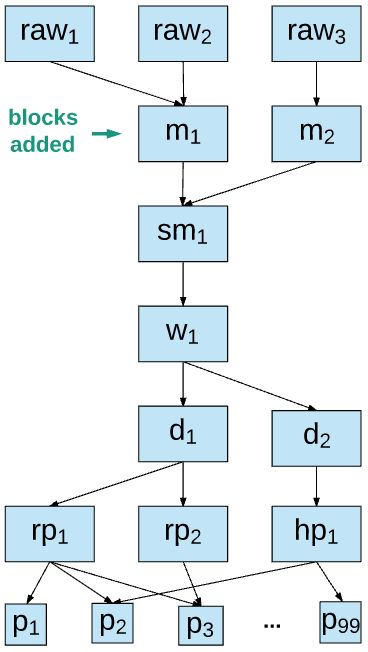
\includegraphics[width=0.5\columnwidth]{images/supply-chain-model.JPG}
  \caption{The flow chart for a pharmaceutical supply chain}\label{f:supplychainmodel}
\end{figure}

\begin{figure}[!ht]
 \centering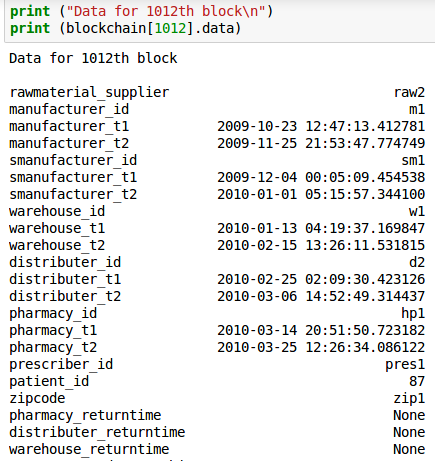
\includegraphics[width=0.75\columnwidth]{images/block_data.png}
  \caption{The data fields that are stored in a block}\label{f:datainablock}
\end{figure}

\begin{figure}[!ht]
 \centering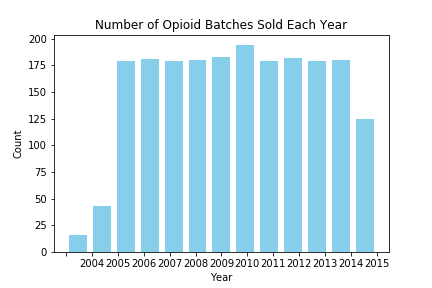
\includegraphics[width=0.75\columnwidth]{images/yearly_batch_count_hist.png}
  \caption{Number of opioid batches sold each year}\label{f:yearlyhist}
\end{figure}

\begin{figure}[!ht]
 \centering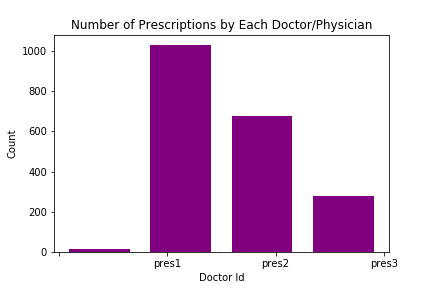
\includegraphics[width=0.75\columnwidth]{images/prescriptions_hist.png}
  \caption{Number of prescriptions by each doctor/physician}\label{f:preshist}
\end{figure}

\begin{figure}[!ht]
 \centering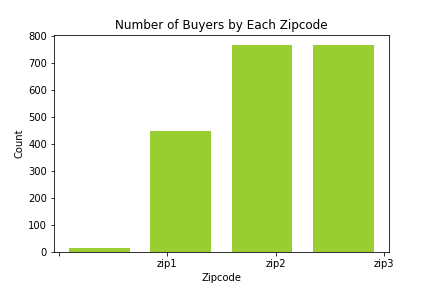
\includegraphics[width=0.75\columnwidth]{images/zipcode_hist.png}
  \caption{Number of buyers by each zipcode}\label{f:ziphist}
\end{figure}

\begin{figure}[!ht]
 \centering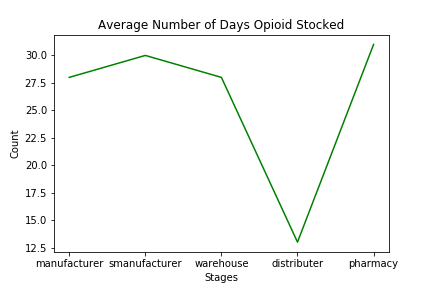
\includegraphics[width=0.75\columnwidth]{images/average_hist.png}
  \caption{Average number of days opioid stocked}\label{f:avghist}
\end{figure}

\end{document}
